\chapter{Đồ thị web và thuật toán PageRank}
%-----------------------------------------------------------------------
%%%%%%%%%%%%%%%%%%%%%%%%%%%%%%%%%%%%%%%%%%%%%%%%%%%%%%%%%%%%%%%%%%%%%%%%
%-----------------------------------------------------------------------
\section{Đồ thị web và xây dựng thuật toán}
\emph{Web graph} hay đồ thị web là một khái niệm được xây dựng để mô tả cấu trúc của \emph{World Wide Web}. Đây là một đồ thị có hướng với quy mô cực lớn, với các node đại diện cho các trang web và các cạnh đại diện  liên kết giữa những trang web với nhau. \emph{Web graph} giúp ta hình dung cụ thể hơn về cách mà các trang web được liên kết với nhau trên Internet. Mỗi trang web có thể chứa các liên kết đến những trang web khác, tạo thành một mạng lưới phức tạp của thông tin trên Internet. Việc phân tích \emph{web graph} đóng vai trò quan trọng trong việc xây dựng thuật toán tìm kiếm và đánh giá trang web mà ở đây là thuật toán PageRank.
\begin{align}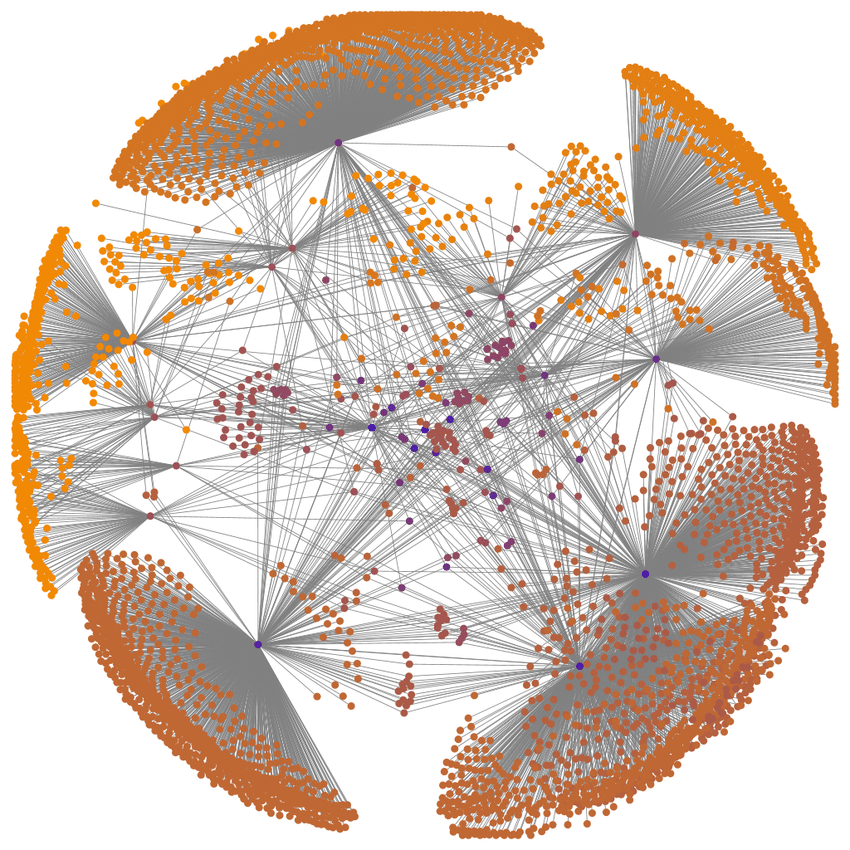
\includegraphics[width=.3\textwidth]{figure/pagerank-example3.png}\end{align}
Để dễ quan sát sự liên kết giữa đồ thị web và làm thế nào hình thành thuật toán PageRank cơ bản cũng như thực hiện các ví dụ, chúng ta có thể quan sát một mô hình nhỏ mô phỏng cho đồ thị web như sau:
\begin{align}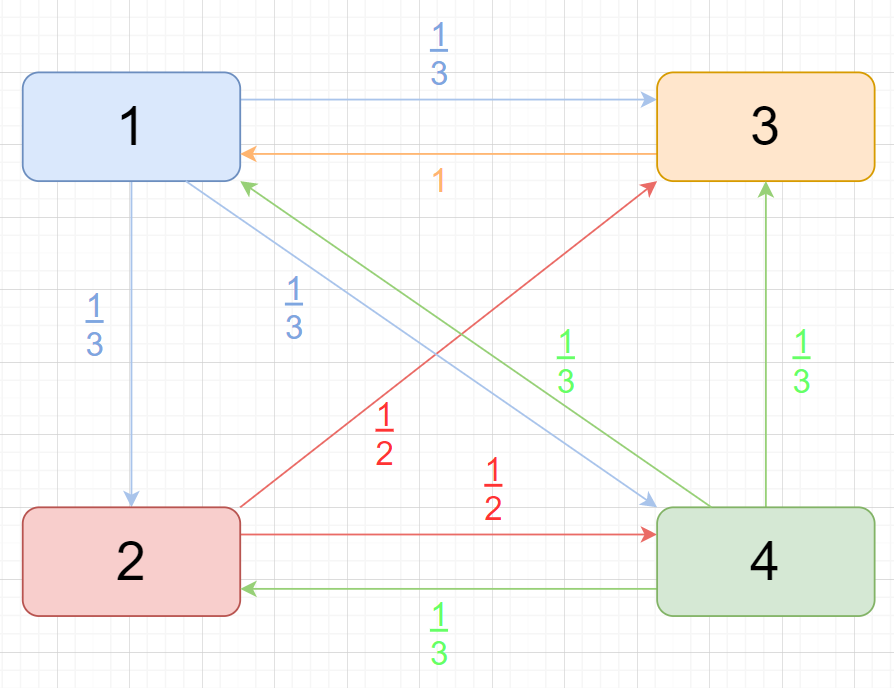
\includegraphics[width=.5\textwidth]{figure/pagerank-example4.png}\end{align}
\textbf{Ví dụ 1:} Trong hình, ta thấy các liên kết: trang web 1 liên kết đến 2, 3, 4; trang web 2 liên kết đến 3, 4; trang web 3 liên kết đến 1; trang web 4 liên kết đến 1, 2, 3. Các con số gắn với mỗi đường liên kết là xác suất mà một mô hình ngẫu nhiên sẽ truy cập qua đường đó đến trang web tiếp theo khi nó đang ở trang web ban đầu. Vậy, ở trang web 1, nơi có liên kết đến cả 3 trang còn lại thì tỉ lệ nhảy đến các trang sẽ chia đều cho nhau và bằng $\displaystyle\frac{1}{3}$.
%-----------------------------------------------------------------------
%%%%%%%%%%%%%%%%%%%%%%%%%%%%%%%%%%%%%%%%%%%%%%%%%%%%%%%%%%%%%%%%%%%%%%%%
%-----------------------------------------------------------------------
\section{Xây dựng thuật toán PageRank}
Tóm lại, thông qua những khái quát về cách mà thuật toán PageRank hoạt động, ta thấy nó được xây dựng bằng cách tận dụng cấu trúc liên kết của Internet - cấu trúc mà có thể mô phỏng ở dạng một đồ thị có hướng - để xây dựng và hình thành nên thuật toán sử dụng một mô hình ngẫu nhiên để đánh giá mức độ \textbf{quan trọng} của một trang web.\newline\newline
Ta có công thức tổng quát để tính rank của trang web dựa vào các trang liên kết đến nó:$$\boxed{r_j = \displaystyle\sum_{i \to j}^{}{\displaystyle\frac{r_i}{d^+(i)}}}$$
\noindent Trong đó:
\begin{itemize}
    \item $r_i$ giá trị PageRank của trang web $i$ có liên kết đến $j$
    \item $r_j$ giá trị PageRank của trang web $j$ 
    \item $d^{+}(i)$ là số lượng \emph{outgoing links} từ trang web $i$
\end{itemize}
\textbf{Ví dụ 2}: Áp dụng công thức tính Rank cho trang web ở trên cho ví dụ ở hình (2.2), ta có PageRank của các trang web được tính như sau: \\
$
\begin{cases}
     r_1 &= r_3 + \dfrac{r_4}{3}\\[10pt]
     r_2 &= \dfrac{r_1}{3} + \dfrac{r_4}{3}\\[10pt]
     r_3 &= \dfrac{r_1}{3} + \dfrac{r_2}{2} + \dfrac{r_4}{3}\\[10pt]
     r_4 &= \dfrac{r_1}{3} + \dfrac{r_2}{2}\\[10pt]
\end{cases}\\
$\\
Và $r_1 + r_2 + r_3 + r_4 = 1$.\\[10pt]
Ta được nghiệm: $r_1 = \dfrac{15}{44}$, $r_2 = \dfrac{2}{11}$, $r_3 = \dfrac{3}{11}$, $r_4 = \dfrac{9}{44}$.\\[10pt]
\indent Đối với bài toán tính PageRank cho các trang web trong trường hợp thực tế, phương pháp giải hệ phương trình hay lược bỏ Gaussian sẽ không còn đơn giản. Vì vậy ta có cách giải quyết tối ưu và hợp lý hơn cho vấn đề này bằng cách sử dụng phương pháp \emph{tính xấp xỉ nghiệm của hệ phương trình này sau 1 số hữu hạn vòng lặp}.

%-----------------------------------------------------------------------
%%%%%%%%%%%%%%%%%%%%%%%%%%%%%%%%%%%%%%%%%%%%%%%%%%%%%%%%%%%%%%%%%%%%%%%%
%-----------------------------------------------------------------------
\section{Xấp xỉ nghiệm}
 Ta sẽ thực hiện xấp xỉ nghiệm mà ở đây sẽ áp dụng phương pháp lặp Seidel áp dụng cho biểu thức dạng $Ax=0$. Cụ thể, thay vì thực hiện tìm nghiệm, ban đầu ta sẽ chọn $x^{(0)}$ nào đó làm nghiệm của phương trình và tính các nghiệm gần đúng tiếp theo $x^{(1)}, x^{(2)}, x^{(3)}, ...$ theo phương pháp lặp đơn sử dụng hệ phương trình mà ta đã lập được từ trước. Khi đó, ta sẽ lặp lại việc tìm kiếm nghiệm đến khi giá trị tạo ra đạt được sự hội tụ, nghĩa là thỏa mãn với yêu cầu mà ta đặt ra từ ban đầu cho bài toán.\\\\
\textbf{Ví dụ 3}: Cụ thể, áp dụng cho ví dụ 2 ở trên, ta chọn giá trị ban đầu là:\\
$$r_1(0)=r_2(0)=r_3(0)=r_4(0)=\displaystyle\frac{1}{4}.$$
\textbf{Vòng lặp thứ 1:}
\begin{enumerate}
    \item $r_1(1) = r_3(0) + \displaystyle\frac{r_4(0)}{3} = \dfrac{1}{4} + \dfrac{1}{12} = \dfrac{1}{3}$
    \item $r_2(1) = \dfrac{r_1(0)}{3} + \dfrac{r_4(0)}{3} = \dfrac{1}{12} + \dfrac{1}{12} = \dfrac{1}{6}$
    \item $r_3(1) = \dfrac{r_1(0)}{3} + \dfrac{r_2(0)}{2} + \dfrac{r_4(0)}{3} = \dfrac{1}{12} + \dfrac{1}{8} + \dfrac{1}{12} = \dfrac{7}{24}$
    \item $r_4(1) = \dfrac{r_1(0)}{3} + \dfrac{r_2(0)}{2} = \dfrac{1}{12} + \dfrac{1}{8} = \dfrac{5}{24}$
\end{enumerate}
\textbf{Vòng lặp thứ 2:}
\begin{enumerate}
    \item $r_1(2) = r_3(1) + \dfrac{r_4(1)}{3} = \dfrac{13}{36}$
    \item $r_2(2) = \dfrac{r_1(1)}{3} + \dfrac{r_4(1)}{3} = \dfrac{13}{72}$
    \item $r_3(2) = \dfrac{r_1(1)}{3} + \dfrac{r_2(1)}{2} + \dfrac{r_4(1)}{3} = \dfrac{19}{72}$
    \item $r_4(2) = \dfrac{r_1(1)}{3} + \dfrac{r_2(1)}{2}  = \dfrac{7}{36}$
\end{enumerate}
...\newline
\textbf{Vòng lặp thứ 40:}
\begin{enumerate}
    \item $r_1(40) = r_3(39) + \dfrac{r_4(39)}{3} = \dfrac{15}{44}$
    \item $r_2(40) = \dfrac{r_1(39)}{3} + \dfrac{r_4(39)}{3} = \dfrac{2}{11}$
    \item $r_3(40) = \dfrac{r_1(39)}{3} + \dfrac{r_2(39)}{2} + \dfrac{r_4(39)}{3} = \dfrac{3}{11}$
    \item $r_4(40) = \dfrac{r_1(39)}{3} + \dfrac{r_2(39)}{2}  = \dfrac{9}{44}$
\end{enumerate}

Ta sẽ thực hiện lặp lại các vòng lặp cho đến khi đạt được sự hội tụ mà thỏa mãn yêu cầu ta đã quy ước từ trước. Giả sử ta có quy ước $\delta = r(n) - r(n-1)$ và $\delta < 1.10^{-5}$ thì ta sẽ thực hiện đến khi giá trị $\delta$ thỏa mãn điều kiện đó. Như ở trên, ở vòng lặp thứ 40, kết quả trả về tương đương với kết quả ở cách tính toán thông thường.